\documentclass{article}

% Language setting
% Replace `english' with e.g. `spanish' to change the document language
\usepackage[english]{babel}


% Set page size and margins
% Replace `letterpaper' with `a4paper' for UK/EU standard size
\usepackage[a4paper, top=2cm,bottom=2cm,left=3cm,right=3cm,marginparwidth=1.75cm]{geometry}

% Useful packages
\usepackage{amsmath,amsfonts}
\usepackage{graphicx,caption}
\usepackage{authblk}
\usepackage{float}
\usepackage[colorlinks=true, allcolors=blue]{hyperref}
\usepackage{natbib}
\usepackage{indentfirst}
\usepackage{amsmath}
% \usepackage{palatino}

\title{A Mathematical Model for Human Fecundability and Aneuploidy-driven Pregnancy Loss}

\author[1]{Arjun Biddanda}
\author[1]{Sara A. Carioscia}
\author[1]{Rajiv C. McCoy}
\affil[1]{Department of Biology, Johns Hopkins University}

\begin{document}
\maketitle

\section*{Model Description}

In the original model from \citep{Macklon2002-zn}, the ``iceberg'' of pregnancy loss probabilities is framed as the \textit{absolute} probability of the pregnancy loss outcome (\ref{fig:1}). However, in many ways it may be more favorable to model the series of \textit{conditional} probabilities that underlie each section of the iceberg. 

\begin{figure}[H]
\begin{center}
    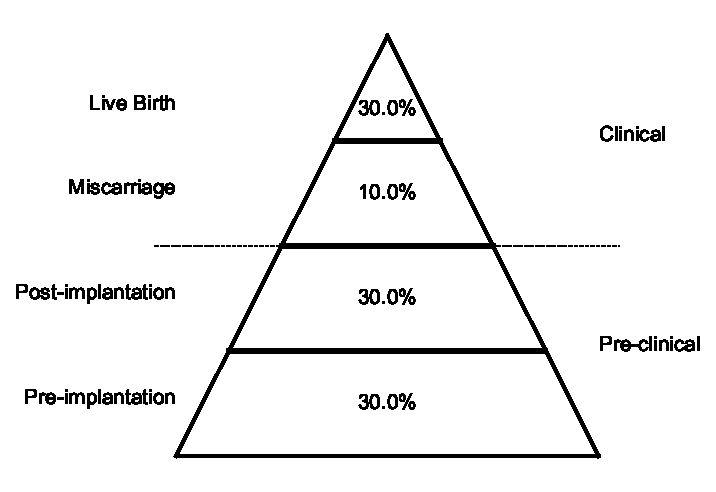
\includegraphics[width=0.5\textwidth]{figures/macklon_recreate.041724.pdf}
\end{center}
\vspace{-1.5em}
\caption{The ``Iceberg'' of pregnancy loss (repurposed from \citep{Macklon2002-zn}).}
\label{fig:1}
\end{figure}

We provide an introduction to the model below, with the conditional probabilities. The  probability we would like to model is the probability of a \textit{live birth conditional on conception occurring}. We model this using a series of conditional probabilities: 

\begin{equation}
	P(\text{Live Birth}) =  (1 - P(\text{Miscarriage} | \text{no EPL})) \cdot (1 - P(\text{EPL} | \text{implantation})) \cdot (1 - P(\text{failed implantation}))
\end{equation}

This model posits that a health live birth (conditional on conception occurring) is conditional on no implantation failure, no early pregnancy loss, \textit{and} no miscarriages.

While there may be a number of potential factors influencing both of these negative events during pregnancy, we primarily focus on the assumption that aneuploidy drives a large fraction of these effects. We first posit that the distribution of aneuploidy outcomes come from the following distribution $P(A,M)$: 

\begin{table}[H]
\begin{center}
	\begin{tabular}{ |c|c|c| } 
	 \hline
	  & Meiotic & Euploid  \\ 
	 \hline
	 None & $\frac{294}{909}$ & $\frac{206}{909}$ \\ 
	 \hline
	 Early-Mitotic & $\frac{260}{909}\times \frac{3}{4}$ & $\frac{(88 + 61)}{909}\times \frac{3}{4}$ \\
	 \hline
	 Late-Mitotic & $\frac{260}{909}\times \frac{1}{4}$ & $\frac{(88 + 61)}{909}\times \frac{1}{4}$\\
	 \hline
	\end{tabular}
	\caption{Joint probability distribution of meiotic (columns) and mitotic (rows) aneuploidy based on outcome data from \citep{McCoy2023-dg}.}
	\label{table:1}
	\end{center}
\end{table}

We have chosen specifically to model the joint distribution of \textit{both} mitotic and meiotic aneuploidies since they both contribute to early pregnancy loss (particular meiotic aneuploidies and early-mitotic aneuploidies). We note that we have also roughly approximated a ratio of 3:1 of early to late-mitotic errors as the first cell divisions post-fertilization are those that are most prone to errors \citep{Currie2022-wp}. As long as the joint probability distribution $P(A,M)$ satisfies being a full probability distribution, then all of the subsequent modeling can be worked through(see later section on scaling for maternal age). 

\subsubsection*{Implantation Failure}

The second conditional model is the implantation failure rate conditioned on aneuploidy type: 

\begin{equation}
P(\text{failed implantation} | A=a, M=m) = \begin{cases}
0.16 &, a = \text{Euploid}, m = \text{None}\\
0.36 &, a = \text{Meiotic}, m = \text{None}\\
0.57 &, a = \text{Euploid}, m = \text{Early-Mitotic}\\
0.55 &, a = \text{Meiotic}, m = \text{Early-Mitotic}\\
0.16 &, a = \text{Euploid}, m = \text{Late-Mitotic}\\
0.36 &, a = \text{Meiotic}, m = \text{Late-Mitotic}\\
\end{cases}
\end{equation}

This conditional probability suggests that different forms of aneuploidy have different impacts on implantation - roughly corresponding to when they arise during development (e.g. meiotic-origin being the earliest).  We have approximated the rate of implantation failure here as the probability of embryo arrest from \citep{McCoy2023-dg} (Figure 4B) -- however there may be other reasons beyond aneuploidy for implantation to fail. We also note that in this model the conribution of later-occurring \textit{mitotic} aneuploidies are effectively limited.   

We can then calculate the following absolute probability:

\begin{equation}
P(\text{failed implantation}) = \gamma_{implant} + \sum_{A}\sum_{M} P(\text{failed implantation} | A, M) P(A, M) ,
\end{equation}

which directly corresponds to the bottom section of the iceberg in \citep{Macklon2002-zn}, but importantly now incorporates different types of aneuploidy. We have also added an intercept term ($\gamma_{implant}$) that captures non-aneuploidy driven pregnancy losses that can occur at this stage.   

\subsubsection*{Early Pregnancy Loss}

We now turn to the second conditional probability for early pregnancy loss (EPL) which is when there is pregnancy loss following a successful implantation but prior to being a clinically-defined miscarriage:

\begin{equation}
	P(EPL | \text{implantation}, A=a, M=m) = \begin{cases}
	\epsilon &, a= \text{Euploid}, m=\text{None}\\
	1 - \eta &, a = \text{Meiotic}, m=\text{None}\\
	1 - \eta &, a = \text{Euploid}, m=\text{Early-Mitotic}\\
	1 - \eta &, a = \text{Meiotic}, m=\text{Early-Mitotic}\\
	\epsilon &, a = \text{Euploid}, m=\text{Late-Mitotic}\\
	1 - \eta &, a = \text{Meiotic}, m=\text{Late-Mitotic}\\
	\end{cases},
\end{equation}

where $\eta$ is an "escape" probability where a meiotic or mitotic aneuploidy does not lead to early-pregnancy loss and $\epsilon$ is the probability of lethal mutations that may lead to early pregnancy loss outcomes even within a euploid embryo (or euploid + late mitotic embryo). The probability of 0.57 comes from \citep{Gu2021-tk} which investigated the aneuploidy status of products of conception \footnote{The parameter $\epsilon$ represents the probability of smaller scale, but still lethal, structural variants so can be thought of as a larger catch-all for lethal mutations that survive implantation but still lead to inviability}. 

The corresponding absolute probability for this section of the ``iceberg'' is: 

\begin{equation}
\begin{aligned}
P(EPL) &=  \gamma_{EPL} + \sum_{A}\sum_{M} P(EPL | \text{implantation}, A, M) \\
&\cdot (1 - P(\text{failed implantation} | A, M) - \gamma_{implant})\\ 
&\cdot P(A, M),
\end{aligned}
\end{equation}

where we have again added in a baseline level of non-aneuploidy driven EPL ($\gamma_{EPL}$). 

\subsubsection*{Miscarriage}

The final consideration is the conditional probability of a miscarriage, conditional on surviving beyond EPL and implantation. 

\begin{equation}
	P(Miscarriage | A=a, M=m) = \begin{cases}
	\epsilon_m &, a= \text{Euploid}, m=\text{None}\\
	1 - \eta_m &, a = \text{Meiotic}, m=\text{None}\\
	1 - \eta_m &, a = \text{Euploid}, m=\text{Early-Mitotic}\\
	1 - \eta_m &, a = \text{Meiotic}, m=\text{Early-Mitotic}\\
	\epsilon_m &, a = \text{Euploid}, m=\text{Late-Mitotic}\\
	1 - \eta_m &, a = \text{Meiotic}, m=\text{Late-Mitotic}\\
	\end{cases},
\end{equation}

We have revised this here to approximately include

In most cases however, we do not have strong estimates for whether the miscarriage was the result of an aneuploidy or not. However, in almost all birth cohort datasets the occurrence of miscarriages reflects a strong U-shaped trend  with maternal age \citep{Gruhn2019-al}. 

We then perform a similar marginalization as before - to get the full probability of miscarriage: 

\begin{equation}
\begin{aligned}
P(\text{Miscarriage}) &=  \gamma_{Miscarriage} + \sum_{A}\sum_{M} P(Miscarriage | A,M)\\
&\cdot (1. - P(EPL | \text{implantation}, A, M) - \gamma_{EPL})\\
&\cdot (1 - P(\text{failed implantation} | A, M) - \gamma_{implant})\\ 
&\cdot P(A, M),
\end{aligned}
\end{equation}

\subsubsection*{Accounting for Maternal Age} 

Since maternal age has a well-documented effect on the abundance of \textit{meiotic} aneuploidies, here we focus on how to scale the original $P(A,M)$ distribution such that the distribution of $P(A = \text{Meiotic})$ can scale as a function of maternal age - whereas the rate of mitotic errors will remain constant as a function of age. Corroborating the total proportion of meiotic aneuploid embryos with the fitted probability of meiotic trisomy in \citep{Gruhn2019-al}, we get approximate maternal age of 46.20 to 47.75 years - significantly higher than the realized 38.9 year average maternal age. 

Under the assumption that the mean maternal age of the patients in \citep{McCoy2023-dg} is $\sim 38.9$ years of age, we scale the marginal probability of a meiotic error $P(A) = \sum_M P(A,M)$ by $\alpha_{age} = \frac{P(M | age)}{P(M | age = 38.9)}$ using the fitted model from \citep{Gruhn2019-al}.

\section*{Results}

\subsection*{Modeling Aneuploidy-driven pregnancy loss across maternal age.}

Following these model approximations - we can estimate how aneuploidy occurrence shapes the distribution of pregnancy losses at various stages in development. The resulting output of this model is a way to generate maternal age specific ``icebergs'' for pregnancy loss risk and fecundability, or the tip of the iceberg (\ref{fig:2}). 

\begin{figure}[H]
\begin{center}
    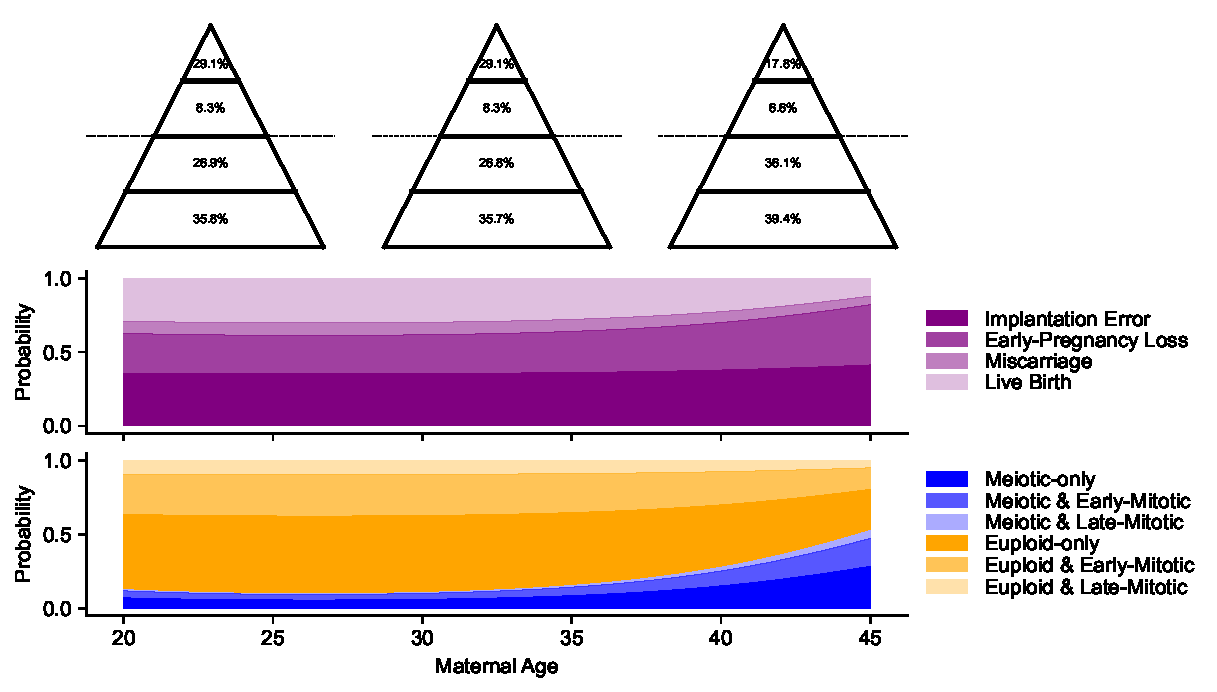
\includegraphics[width=0.75\textwidth]{figures/model_figure.042024.pdf}
\end{center}
\vspace{-1.5em}
\caption{Display of how the rates of aneuploidy are shaped by maternal age (bottom row) and correspondingly shape pregnancy losses at different stages (middle + top row).}
\label{fig:2}
\end{figure}

Importantly, we note that mitotic-origin categories occur at a constant rate as a function of maternal age. 

\subsection*{Relationship to Fecundity and Fecundability}

It is important to note that our model is more closely related to \textit{fecundity} - the probability of a live birth in a given menstrual cycle - than to \textit{fecundability} - the probability of becoming \textit{pregnant} in a given menstrual cycle. We have assumed that the model is conditional on a conception occurring. However, we can also approximate these two quantities using a similar interpretation: 

\begin{equation}
\begin{aligned}
Fecundability &= P(conception)\times (1 - P(\text{Failed implantation}))\\
Fecundity &= P(conception)\times P(\text{Live Birth})
\end{aligned},
\end{equation}

where we have defined here the probability of becoming pregnant as a successful conception \textit{and} implantation occurring. While these two quantities are certainly related - and mediated by aneuploidy of different forms - they also make a clear assumption of what $P(conception)$ is. If we use the approximate estimate of $P(conception) \approx 0.1 - 0.33$ from \citep{Wilcox1995-hs} then we can arrive at  0.13 (0.064, 0.212) for \textit{Fecundability} and 0.048 (0.022, 0.073) for \textit{Fecundity} for a maternal age of 30 years old.

\section*{Discussion + Interpretations}

There are a number of limitations to our modeling here that may warrant further attention. We detail some of these below: 

\begin{enumerate}
\item \textbf{Age-related variation in non-aneuploidy factors}. Currently, we have not modeled an age-dependence on the non-aneuploidy driven factors (e.g. $\gamma_{implant}$) when it is likely that these factors may also have a strong relationship with age. However, in the absence of well-curated epidemiological data to directly model environmental variables and its affect on specific categories of loss, we leave this as an area for future exploration.  
\item \textbf{Relationship between PGT-A and Natural Conceptions}. Most of the basis for understanding embryonic aneuploidy in recent years has been driven by genetic observations from in-vitro fertilization (IVF), which may be potentially a biased representation of what occurs in natural conceptions. For example, due to monetary cost, it is fiscally more reasonable to only assay embryos with a visually better embryo grade - leading to higher-quality embryos being assessed for aneuploidies. For instance, this would make the estimate from \ref{table:1} a potential under estimate of the underlying probability of aneuploidy. If we take this to mean that estimates from PGT-A \textit{underestimate} the probability of aneuploidies in natural conceptions, then implicitly our estimate of fecundability and fecundity are an \textit{upper-bound}. However, it is also possible that estimates of the probability of aneuploidy are upwardly biased in PGT-A due to aspects of IVF being fundamentally different than natural conception, in which case our estimates would be \textit{lower-bounds}. It is worth considering with future data how these experimental biases may be better investigated to improve our broader understanding of fecundability.
\end{enumerate}



\bibliographystyle{plainnat}
\bibliography{refs}

\end{document}
